\documentclass[11pt,a4paper]{article}

\usepackage[utf8]{inputenc}
\usepackage[T1]{fontenc}
\usepackage{lmodern}
\usepackage{geometry}
\usepackage{setspace}
\usepackage{graphicx}
\usepackage{booktabs}
\usepackage{amsmath}
\usepackage{amssymb}
\usepackage{natbib}
\usepackage{hyperref}

\geometry{margin=2.5cm}
\onehalfspacing

\title{GATrESN: An AI-Driven Digital Twin Framework for Strategic Operations Management}
\author{
Cesar H. Valencia\\
Universidad Santo Tom\'as\\
Bucaramanga, Colombia\\
\href{mailto:cesar.valencia@ustabuca.edu.co}{cesar.valencia@ustabuca.edu.co}\\
\href{https://orcid.org/0000-0001-6077-6458}{ORCID: 0000-0001-6077-6458}
\and
Laura M. Valencia\\
Universidade Federal do Rio de Janeiro\\
Rio de Janeiro, Brazil\\
\href{mailto:email@email.edu}{email@email.edu}\\
\href{https://orcid.org/0000-0002-3234-6589}{ORCID: 0000-0002-3234-6589}
}
\date{}

\begin{document}

\maketitle

\begin{abstract}
Strategic operations management increasingly requires decision-support systems capable of representing complex organizational behavior under uncertainty. This paper proposes GATrESN, an AI-driven digital twin framework for strategic operations management that integrates Genetic Algorithms, Transformer-style attention, and Echo State Networks. The framework represents an organization as a dynamic digital model composed of demand, capacity, cost, service-level, utilization, and operational-risk components. A simulation-based case study is developed to evaluate adaptive strategic policies across a multi-site and multi-product operational environment. The proposed approach demonstrates how artificial intelligence can support strategic decision-making by forecasting operational behavior, simulating what-if scenarios, and optimizing strategic alternatives according to performance, cost, risk, and service objectives.
\end{abstract}

\textbf{Keywords:} GATrESN; digital twin; artificial intelligence; echo state network; transformer attention; genetic algorithm; strategic operations management; simulation; decision support

\section{Introduction}
Organizations operate under increasing uncertainty, driven by demand variability, resource constraints, supply disruptions, technological change, and competitive pressure. Strategic operations management must therefore move beyond static planning models and adopt adaptive decision-support systems that connect operational data, predictive intelligence, and scenario-based evaluation.

Digital twins provide a promising mechanism for representing real or conceptual systems in a dynamic computational environment. When combined with artificial intelligence, digital twins can evolve from descriptive replicas into predictive and prescriptive decision-support platforms. In this context, an AI-driven digital twin can support strategic operations management by forecasting future states, simulating strategic alternatives, detecting performance deviations, and recommending adaptive actions.

This paper proposes GATrESN, an AI-driven digital twin framework for strategic operations management. The contribution is threefold: first, it presents a modular architecture connecting organizational data, digital twin modeling, AI analytics, and strategic decision support; second, it integrates Echo State Networks, Transformer-style attention, and Genetic Algorithms into a reproducible strategic decision model; third, it demonstrates the framework through a simulation-based case study implemented in MATLAB.

\section{Literature Background}
\subsection{Digital Twins in Operations Management}
Digital twins have been widely discussed as virtual representations of physical or organizational systems. In operations management, they enable monitoring, simulation, and decision support across production, logistics, maintenance, and service systems.

\subsection{Artificial Intelligence for Strategic Decision Support}
Artificial intelligence techniques, including machine learning, forecasting, anomaly detection, and optimization, can enhance strategic decisions by identifying patterns and estimating future system behavior.

\subsection{Research Gap}
Although digital twins and AI have been studied in operational contexts, there remains a need for integrated frameworks that explicitly connect AI-driven digital twins with strategic operations management. In particular, the literature requires models that link predictive analytics, scenario simulation, and multi-criteria strategic evaluation.

\section{Proposed Framework}
The proposed framework consists of six layers:

\begin{enumerate}
    \item \textbf{Organizational system layer:} represents processes, resources, demand, capacity, costs, and strategic objectives.
    \item \textbf{Data layer:} collects operational indicators such as demand, cycle time, utilization, cost, service level, and risk.
    \item \textbf{Digital twin layer:} creates a computational representation of the operational system and its constraints.
    \item \textbf{AI analytics layer:} applies forecasting, classification, anomaly detection, and performance estimation.
    \item \textbf{Strategic decision layer:} compares strategic scenarios using multi-criteria evaluation.
    \item \textbf{Feedback layer:} updates the model as new operational observations become available.
\end{enumerate}

\section{Methodology}
\subsection{Simulation-Based Case Study}
Due to the conceptual and methodological nature of this study, a synthetic strategic operations dataset is generated to represent realistic organizational behavior under uncertainty. The dataset emulates typical operational patterns involving demand variability, resource constraints, cost fluctuations, capacity utilization, service-level performance, and operational risk.

\subsection{Key Performance Indicators}
The digital twin evaluates each strategy using the following indicators:

\begin{itemize}
    \item Expected demand fulfillment.
    \item Resource utilization.
    \item Operating cost.
    \item Service level.
    \item Strategic risk.
    \item Composite strategic performance score.
\end{itemize}

\subsection{Strategic Scenarios}
Five strategic alternatives are evaluated:

\begin{enumerate}
    \item Conservative strategy.
    \item Efficiency-oriented strategy.
    \item Expansion-oriented strategy.
    \item Resilience-oriented strategy.
    \item AI-adaptive strategy.
\end{enumerate}

\section{GATrESN Computational Model}
Let $D_t$ denote demand at time $t$, $C_t$ operational capacity, $U_t$ resource utilization, $K_t$ operating cost, $S_t$ service level, and $R_t$ operational risk. The digital twin estimates the strategic performance of policy $p$ as:

\begin{equation}
    \text{Score}_{p,t} =
    w_s S_{p,t}
    + w_u (1 - |U_{p,t} - U^*|)
    + w_c (1 - \hat{K}_{p,t})
    + w_r (1 - R_{p,t}),
\end{equation}

where $w_s$, $w_u$, $w_c$, and $w_r$ are decision weights, $U^*$ is the target utilization level, and $\hat{K}_{p,t}$ is normalized cost.

\section{Results}
The MATLAB implementation generates the synthetic enterprise operations dataset, trains the GATrESN forecasting module, optimizes strategic decisions through the Genetic Algorithm, and produces comparative figures for demand forecasting, service level, residual risk, and composite strategic performance.

% Figures will be enabled after running the MATLAB script and generating the PNG files.
% \begin{figure}[htbp]
%     \centering
%     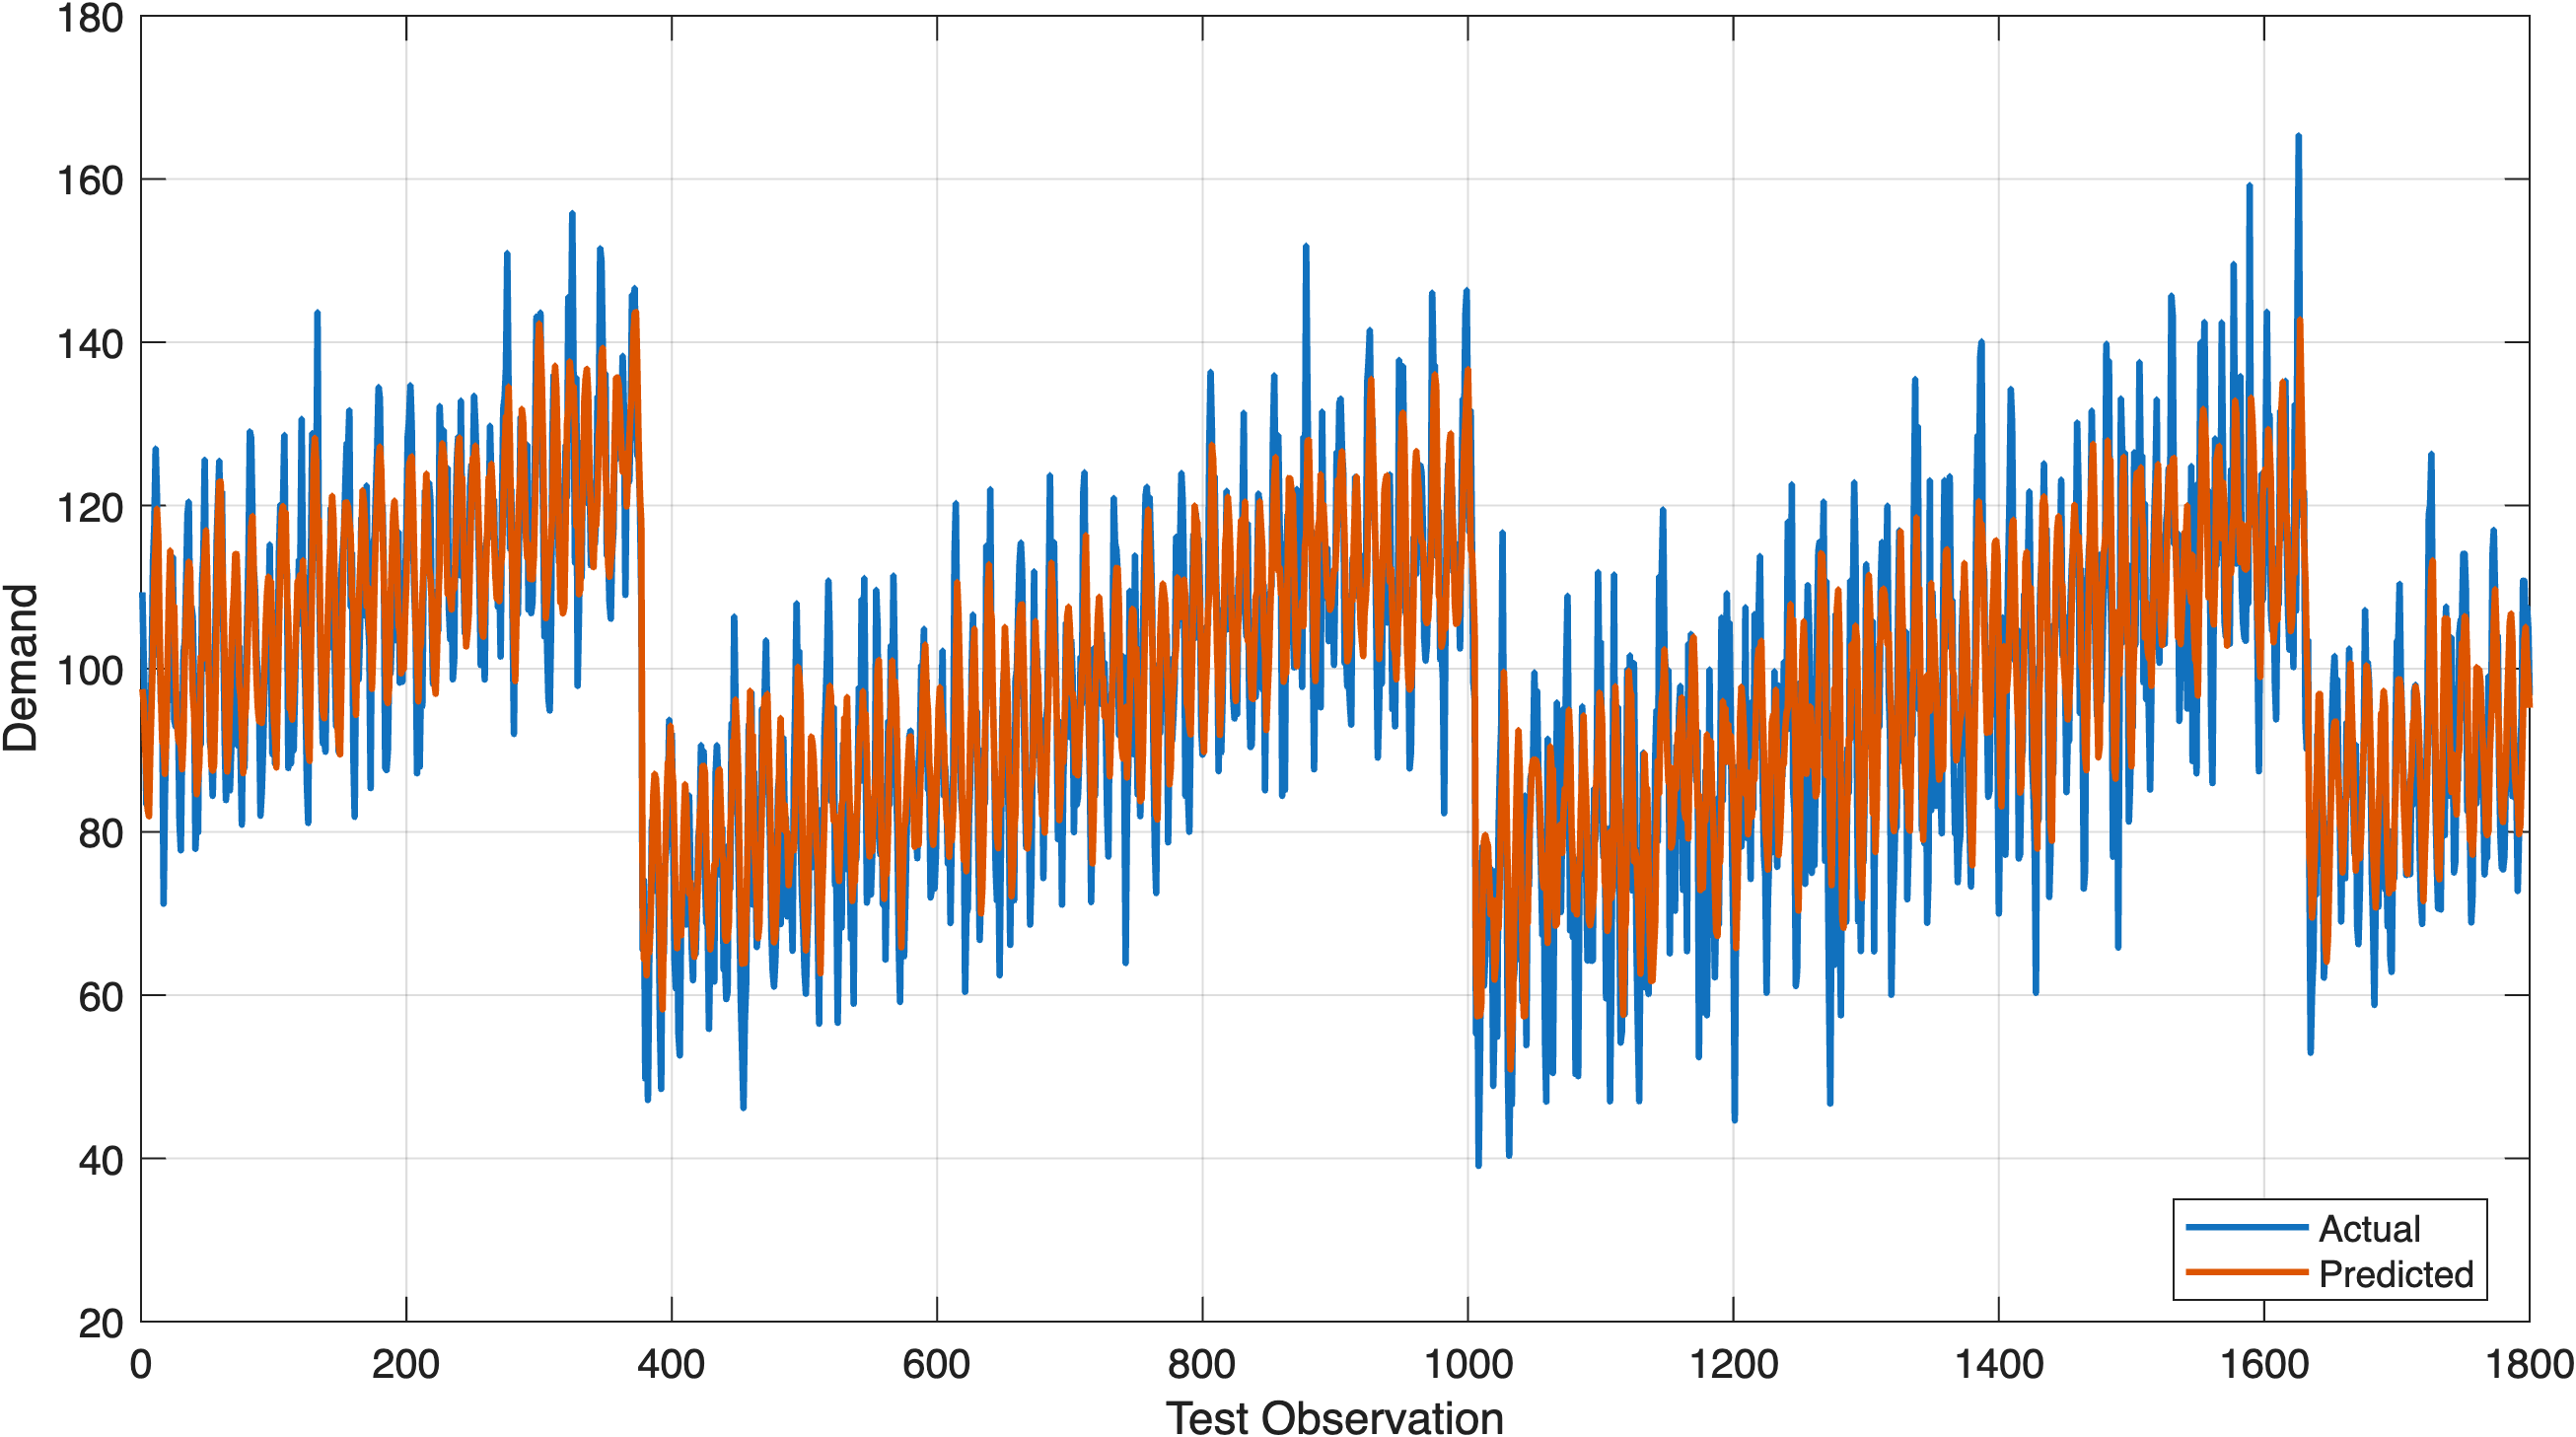
\includegraphics[width=0.90\textwidth]{../figures/GATrESN_demand_forecast.png}
%     \caption{GATrESN demand forecasting performance on the test set.}
%     \label{fig:gatr_esn_forecast}
% \end{figure}
%
% \begin{figure}[htbp]
%     \centering
%     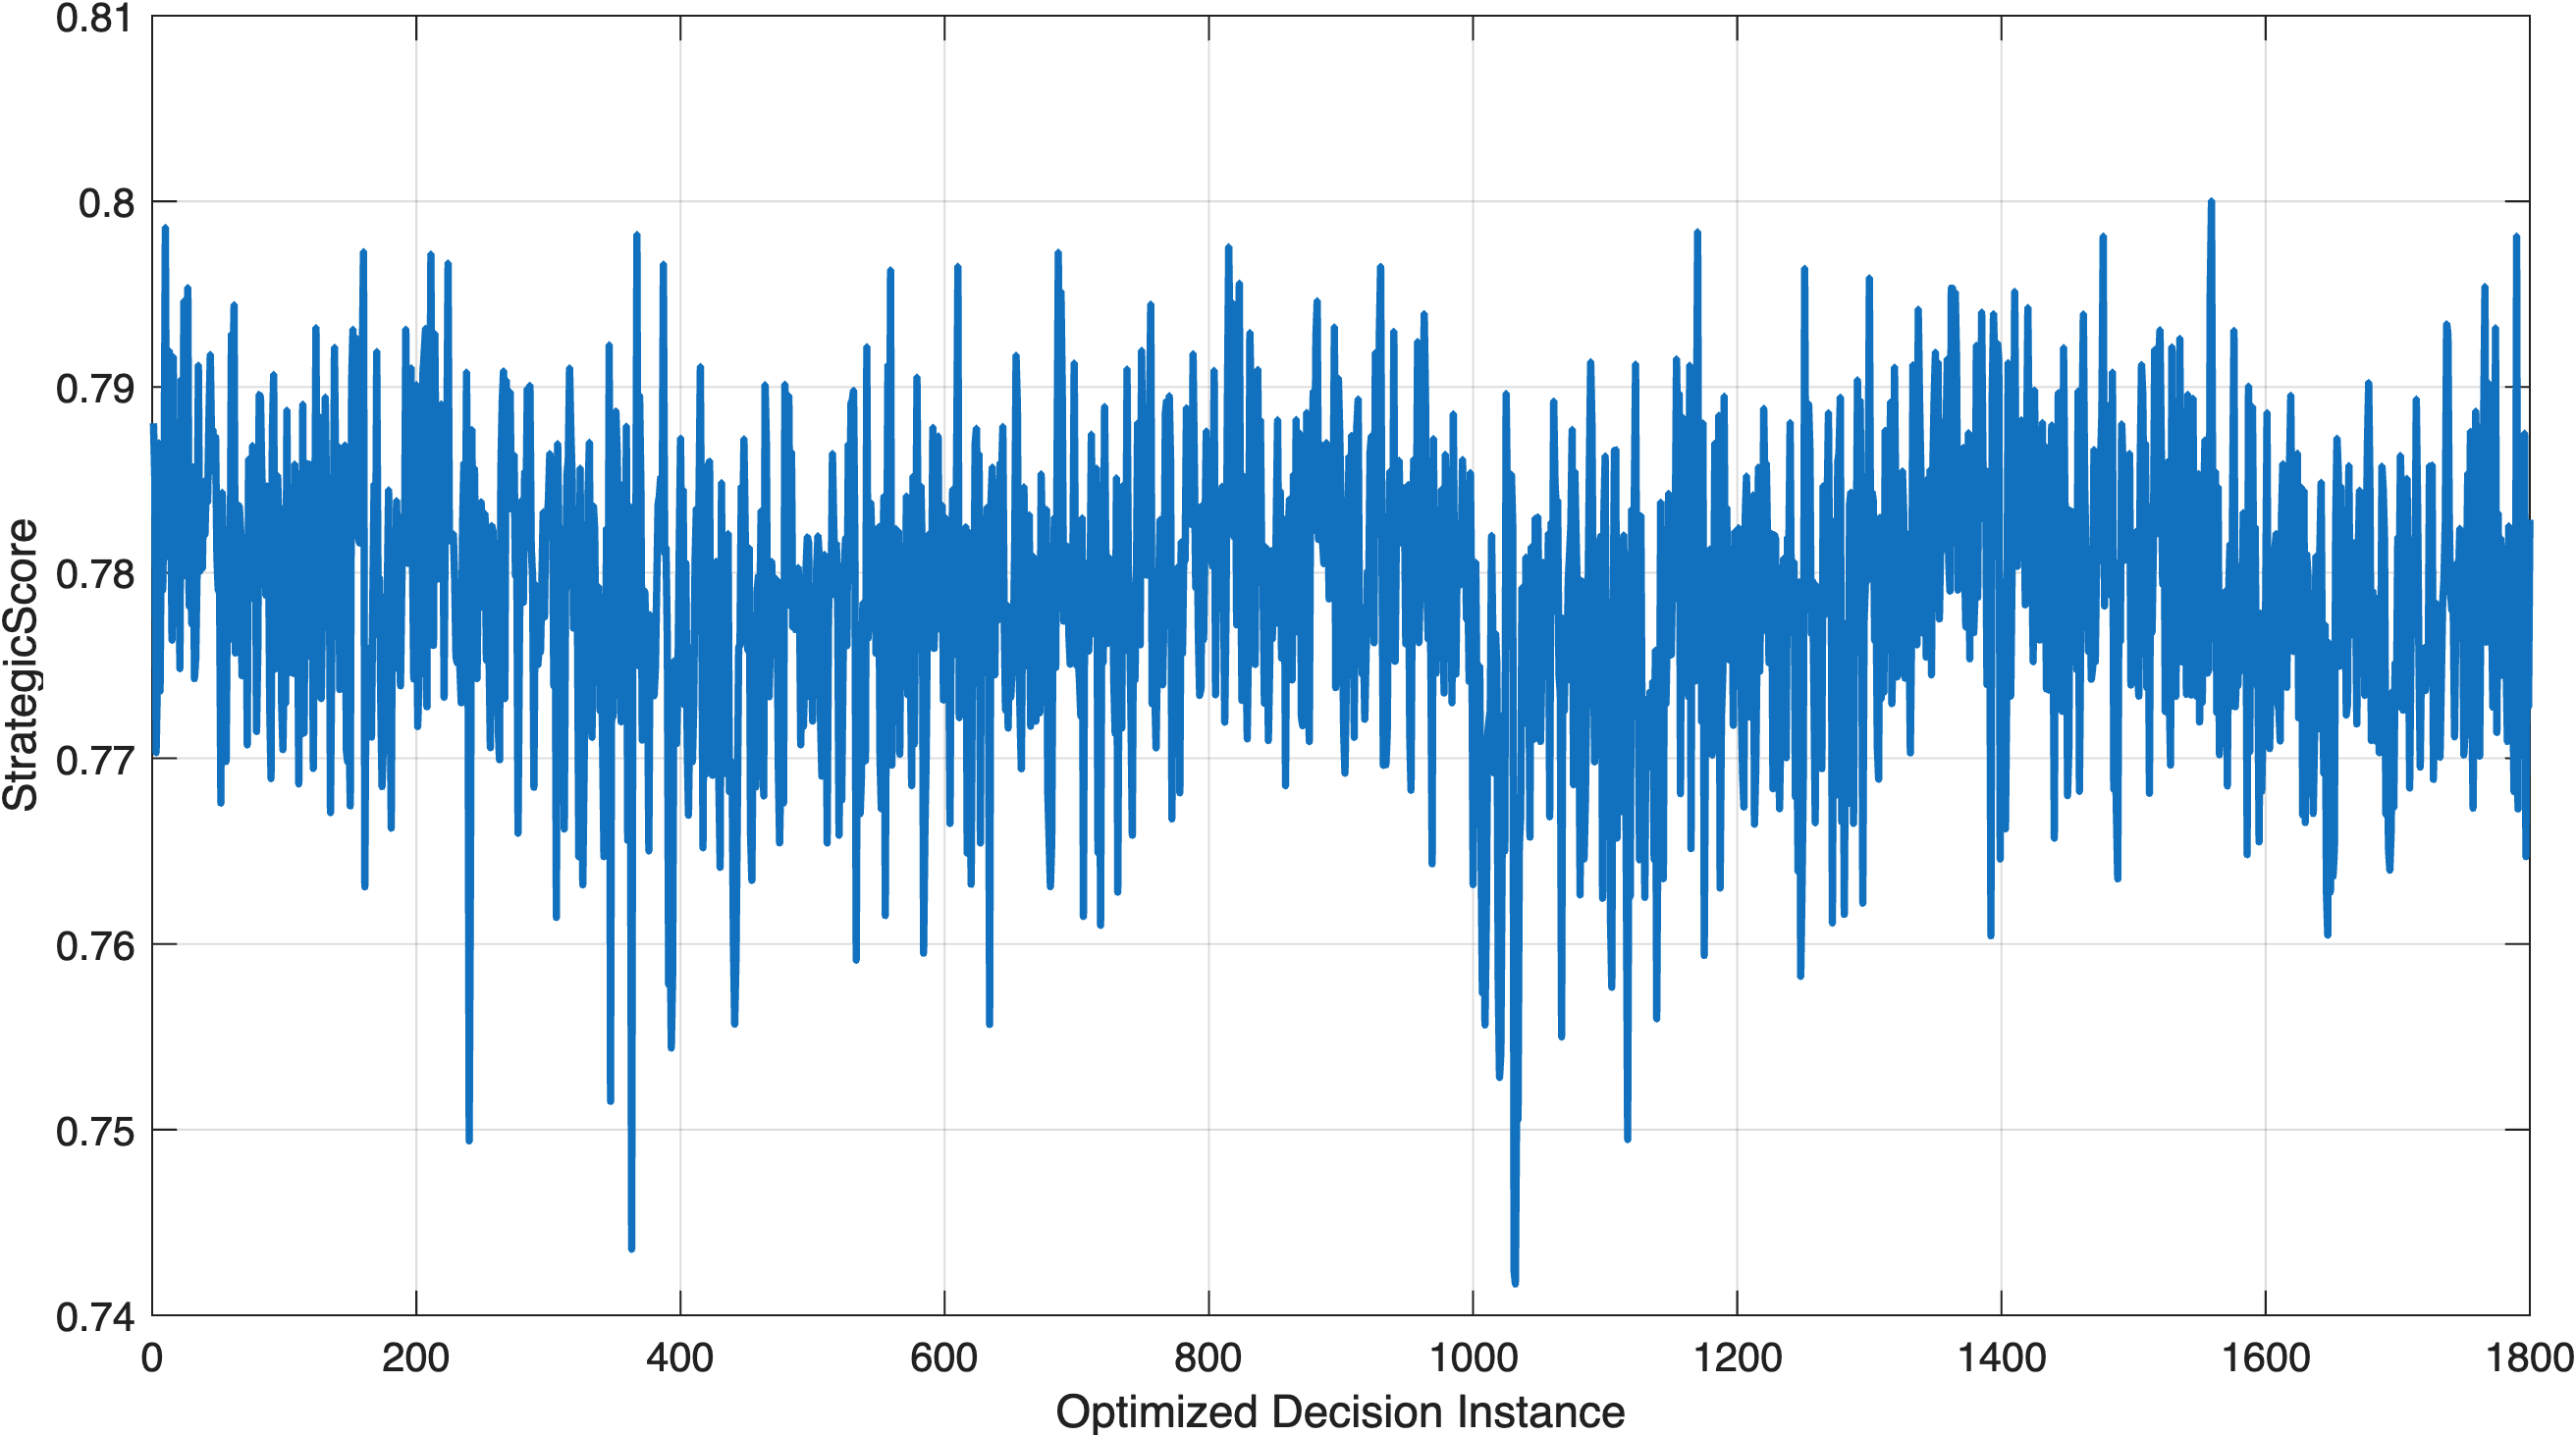
\includegraphics[width=0.90\textwidth]{../figures/GATrESN_strategic_score.png}
%     \caption{GA-optimized strategic performance score generated by the GATrESN digital twin.}
%     \label{fig:gatr_esn_score}
% \end{figure}
%
% \begin{figure}[htbp]
%     \centering
%     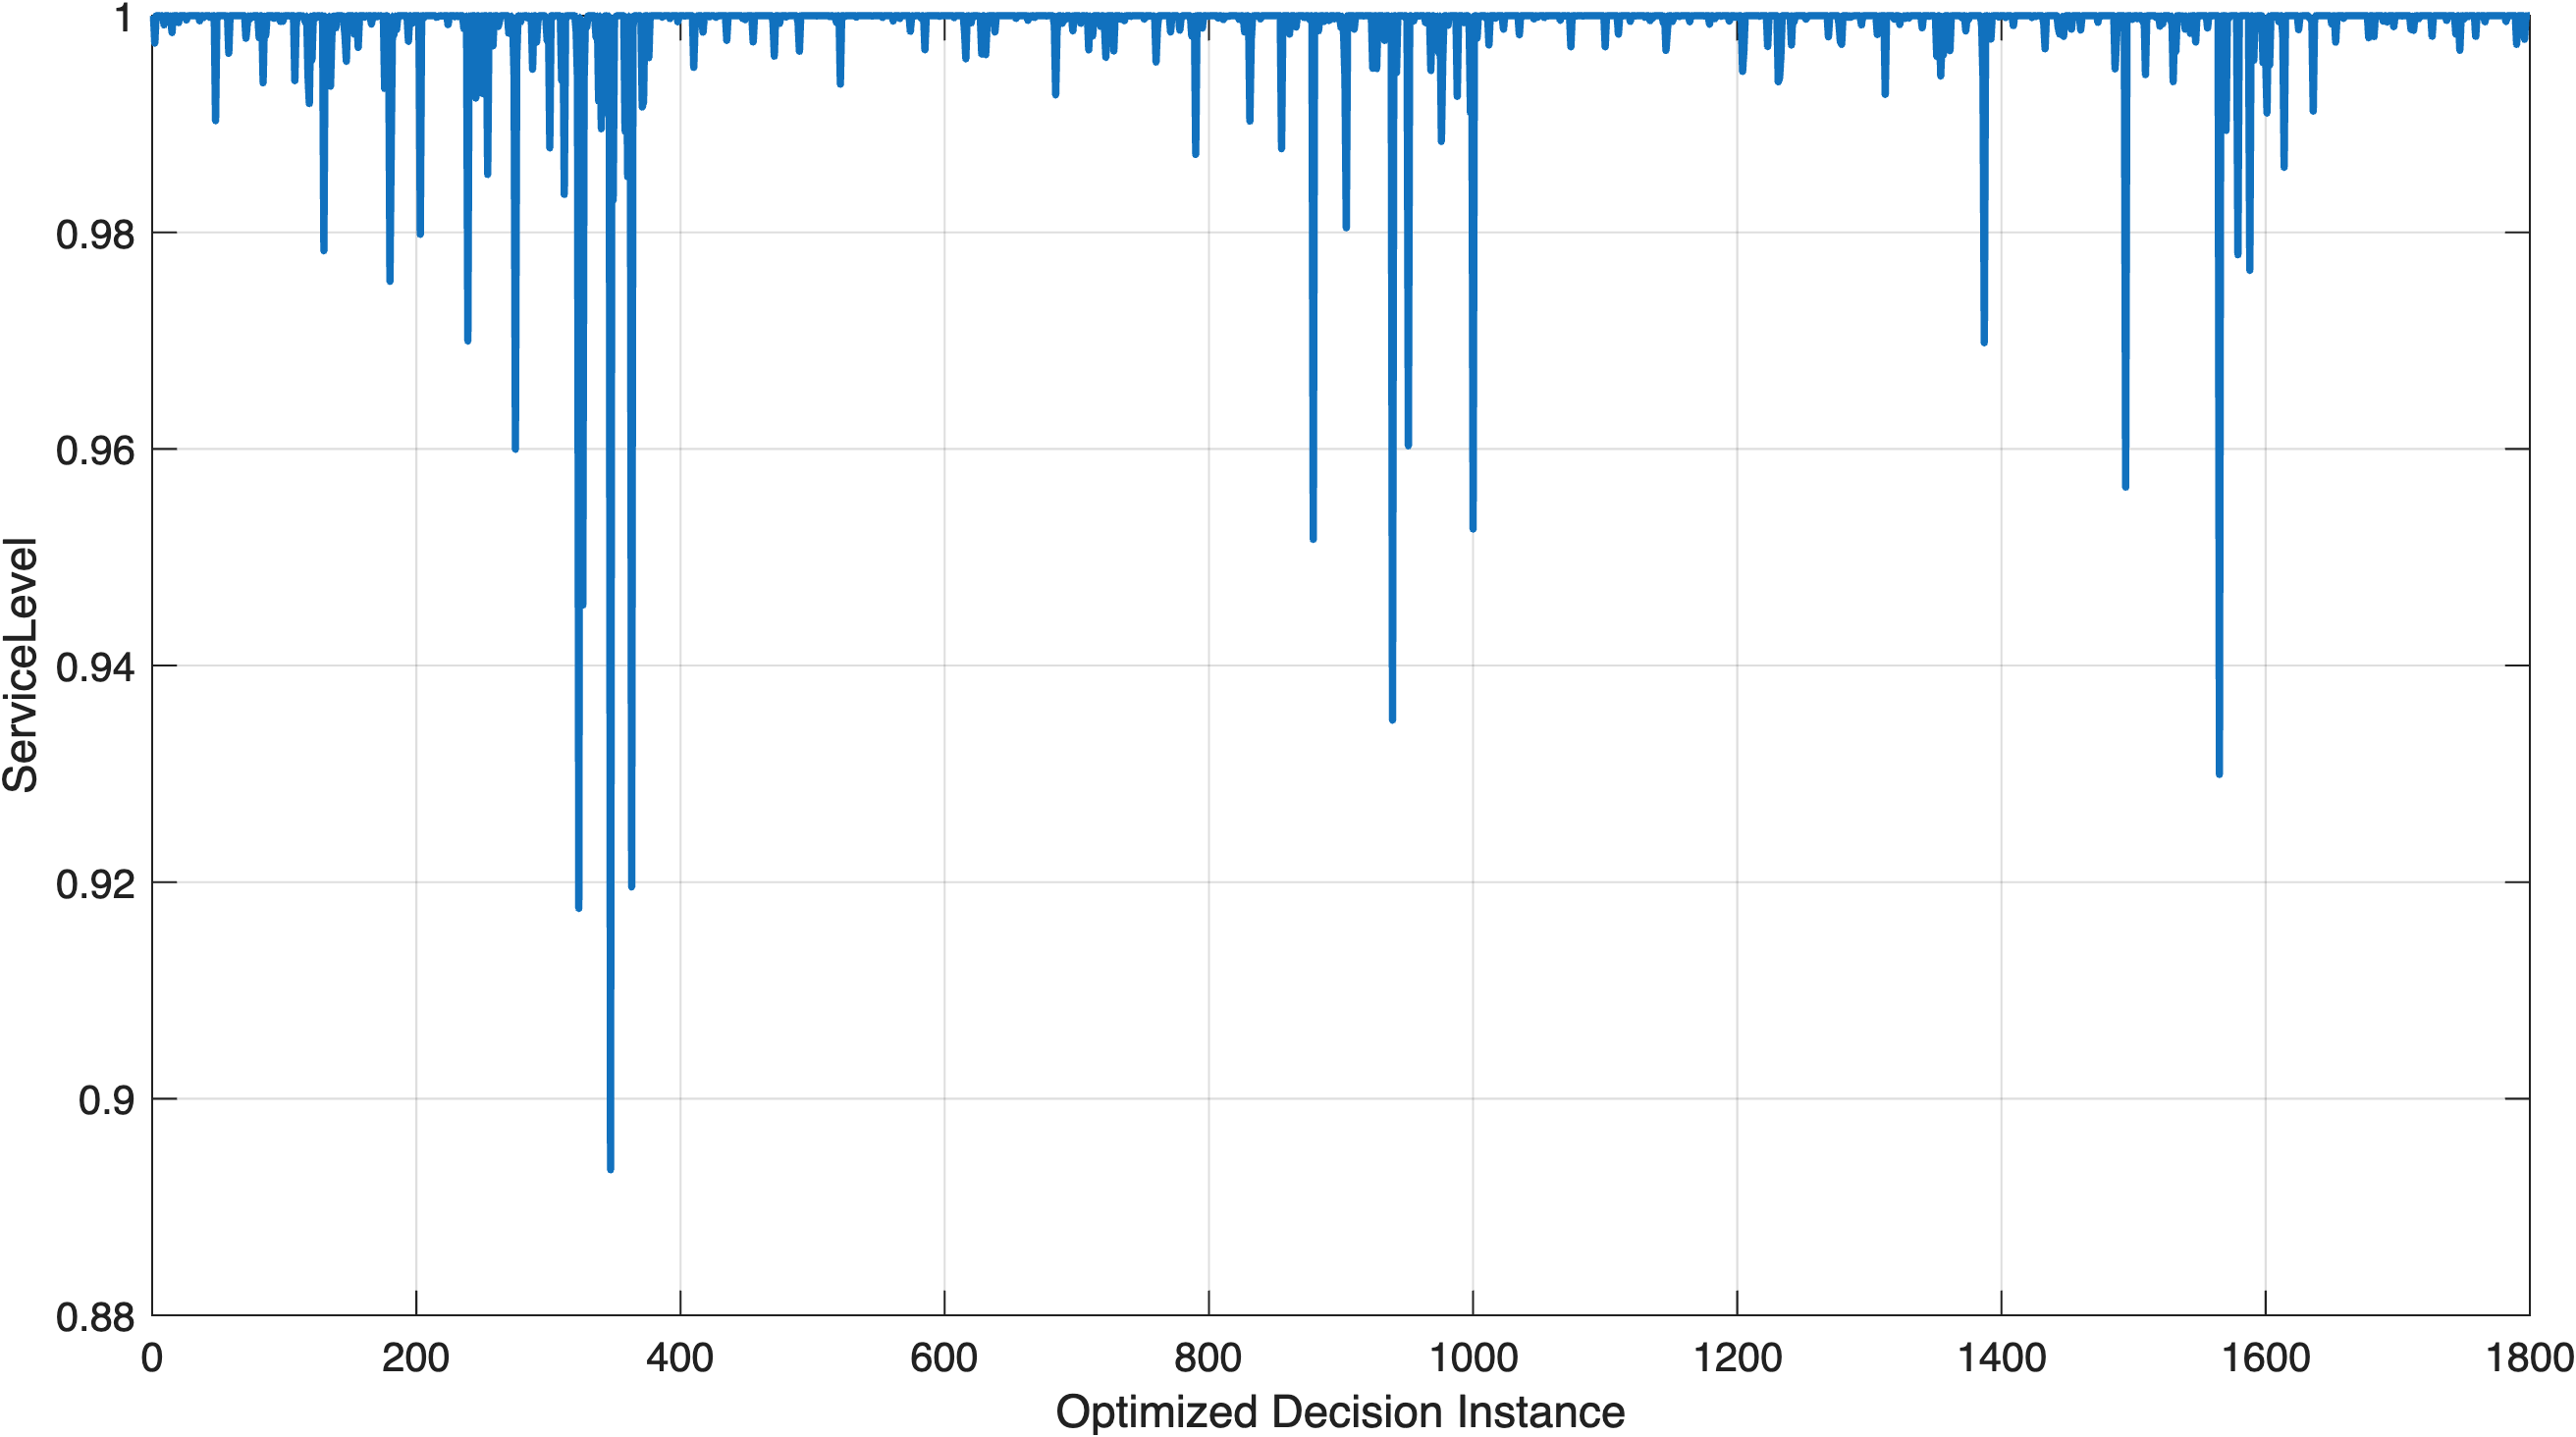
\includegraphics[width=0.90\textwidth]{../figures/GATrESN_service_level.png}
%     \caption{Optimized service-level behavior across decision instances.}
%     \label{fig:gatr_esn_service}
% \end{figure}
%
% \begin{figure}[htbp]
%     \centering
%     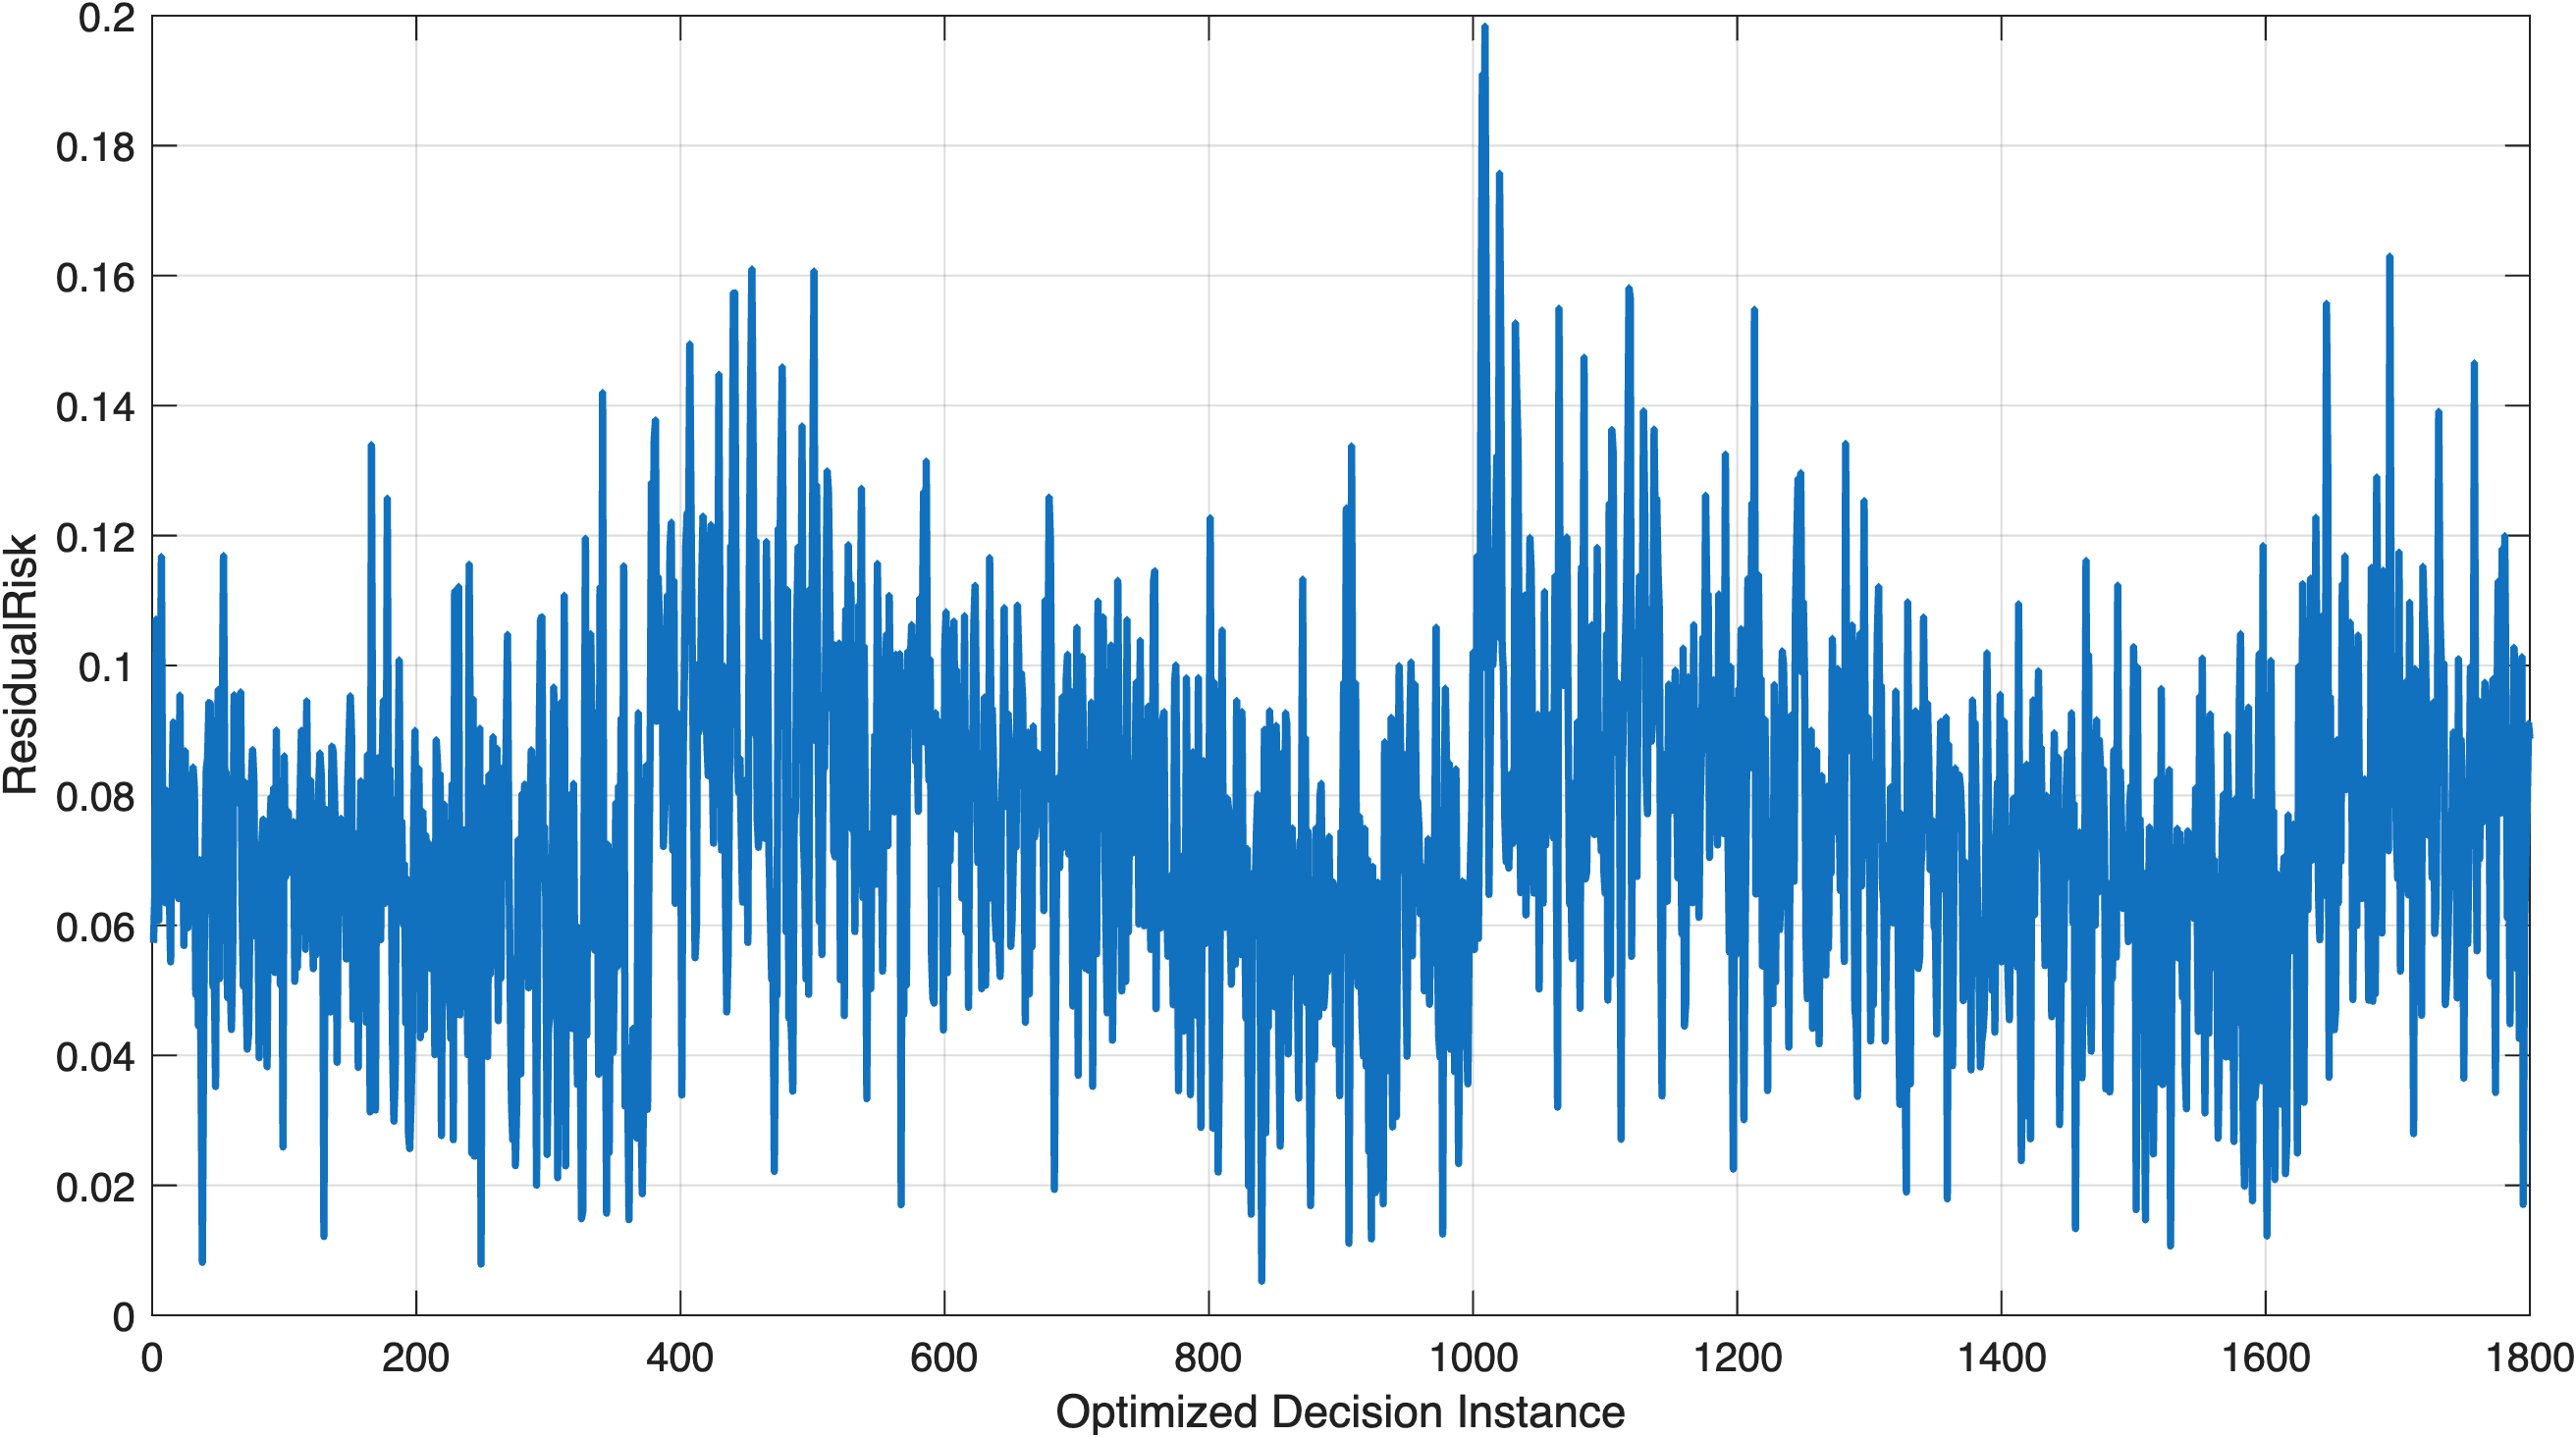
\includegraphics[width=0.90\textwidth]{../figures/GATrESN_residual_risk.png}
%     \caption{Residual operational risk after GA-based resilience optimization.}
%     \label{fig:gatr_esn_risk}
% \end{figure}

The expected result is that the GATrESN strategy improves strategic decision quality under variable demand and uncertainty by dynamically balancing service level, utilization, cost, and operational risk.

\section{Discussion}
The proposed framework illustrates how AI-driven digital twins can support strategic operations management by enabling predictive, scenario-based, and adaptive decision-making. Unlike conventional planning tools, the framework allows decision-makers to test strategies before implementation and evaluate trade-offs across multiple objectives.

\section{Conclusions}
This study presents an AI-driven digital twin framework for strategic operations management and demonstrates its use through a simulation-based case study. The framework integrates digital twin modeling, artificial intelligence, scenario simulation, and multi-criteria decision support. Future research may extend the framework using empirical organizational data, real-time enterprise systems, and explainable AI methods.

\section*{Data Availability Statement}
The data used in this study are synthetically generated for methodological demonstration and reproducibility purposes. The MATLAB code used to generate the dataset and reproduce the simulation results is provided with the manuscript materials.

\section*{Conflicts of Interest}
The author declares no conflict of interest.

\bibliographystyle{plainnat}
\bibliography{../references/references}

\end{document}
